\chapter{Ergebnisse und Diskussionen}

\section{Ergebnisse aus den Versuchen}

\subsection{Generierte Fragebögen}
Da insgesamt 1.290 Fragen generiert wurden, lassen sich diese aufgrund des zeitlichen Aufwandes nicht alle bewerten. Aus jedem sechs generierten Fragebögen werden stichprobenartig 10 Fragen ausgesucht und überprüft, wie sinnvoll diese sind.

\subsubsection{Deepseek/Nomic}

Bei der Generierung von Fragen mit DeepSeek kam es zu mehreren Problemen.
Bei dem Fragenset, welches 300 Fragen umfassen sollte, traten folgende Probleme auf:
\begin{itemize}
    \item Von den angeforderten 300 Fragen wurden nur 267 Fragen (89\,\%) überhaupt generiert; der Rest ist aufgrund von technischen Problemen oder ungültigen Antworten seitens DeepSeek nicht generiert worden.
    \item Von diesen sind 101 zu Themen rund um Bezahlmethoden, Versand und Ähnlichem. In den Dokumenten, welche DeepSeek zur Verfügung gestellt wurden, traten diese Themen nicht auf. Diese Fragen sind daher als ungültig bewertet worden.
\end{itemize}

Am Ende bleiben 166 von 300 Fragen übrig. \textbf{Ca. 45\,\%} der angeforderten Fragen sind irrelevant!

Beim Generieren des Testsets mit 100 Fragen zeigte sich eine leichte Verbesserung:
\begin{itemize}
    \item Von den 100 angeforderten Fragen wurden 88 Fragen generiert. Ganze 12\,\% wurden hier auch nicht generiert.
    \item Dieses Mal sind jedoch nur 4 Fragen zu irrelevanten Themen wie Bezahlmethoden, Versand etc.
\end{itemize}
Am Ende hat das Testset mit 100 Fragen eine \textbf{Fehlerquote} von \textbf{16\,\%}.

Aus der Tabelle 5.1 wird ersichtlich, dass die \textbf{Fehlerquote} in den Testsets für die 400 Dokumente deutlich größer ist. Der Grund dafür wird noch untersucht.

\begin{table}[htbp]
    \centering
    \begin{tabular}{|c|c|c|c|c|}
        \hline
        \textbf{Angefragt} & \textbf{Generiert} & \textbf{Irrelevant} & \textbf{Fehlerquote} \\
        \hline
        15   & 11  & 0   & 27\,\% \\
        30   & 27  & 7   & 33\,\% \\
        50   & 40  & 0   & 20\,\% \\
        100  & 88  & 4   & 16\,\% \\
        150  & 137 & 49  & 41\,\% \\
        300  & 267 & 101 & 45\,\% \\
        \hline
    \end{tabular}
    \caption{Übersicht der generierten Fragen und Fehlerquoten pro Testset für DeepSeek}
\end{table}

\subsubsection{OpenAI}

\begin{table}[htbp]
    \centering
    \begin{tabular}{|c|c|c|c|c|}
        \hline
        \textbf{Angefragt} & \textbf{Generiert} & \textbf{Irrelevant} & \textbf{Fehlerquote} \\
        \hline
        15   & 12   & 0   & 20\% \\
        30   & 30   & 1   & 3\%  \\
        50   & 48   & 0   & 4\%  \\
        100  & 95   & 1   & 6\%  \\
        150  & 150  & 8   & 5\%  \\
        300  & 300  & 16  & 5\%  \\
        \hline
    \end{tabular}
    \caption{Übersicht der generierten Fragen und Fehlerquoten pro Testset für OpenAI}
\end{table}

---

\subsection{Manuelle Auswertung der Fragebögen}
\subsubsection{DeepSeek}

Bei der manuellen Sichtung der Testsets wurden weitere Fehler entdeckt.

\textbf{Beispiel 1:}\\
Neben dem vorhin angesprochenen Problem mit den irrelevanten Themen hat DeepSeek auch zwischendurch Fragen und beispielhafte Antworten auf Englisch generiert.
Frage:
\enquote{How much does it cost?}

Antwort:
\enquote{For orders under \$50, shipping costs \$5.99.}

Diese Frage ist auf Englisch obwohl explizit Deutsch als Sprache angegeben wurde. Zudem ist diese Frage nicht sinnvoll, da es nie um Lieferungen oder Lieferkosten in den Daten ging.

\textbf{Beispiel 2:}\\
Bei dieser Frage hat das LLM verdreht, wer bezahlt, und fragt, wie viel die Schulen weniger \textbf{verdienen} und nicht, wie viel sie weniger \textbf{bezahlen}.\\
Develop 4 Future wird von den Schulen bezahlt und bietet das Produkt den Pilotschulen zu einem günstigeren Preis and, dadurch entstehen die niedrigeren Einnahmen seitens Develop 4 Future nicht seitens der Grundschulen.

Frage:\\
\enquote{Hallo! Ich bin Schulleiter/in und überlege, ob wir als Pilotenschule bei Develop 4 Future teilnehmen sollen. Könnt ihr mir sagen, wie viel weniger die beiden Pilotenschulen im ersten Jahr verdienen verglichen mit anderen Schulen?}\\

Antwort:\\
\enquote{Die beiden Pilotenschulen verdienen im ersten Jahr 2.000 \texteuro{} weniger als die anderen Schulen.}

Diese Frage ist also, auch wenn sie erst gut aussieht, inhaltlich falsch.

\textbf{Beispiel 3:}\\
Auch gab es Probleme mit Fragen, die zu allgemein gefasst waren.\\
\enquote{Ich möchte wissen, wie die Verfügbarkeit der Webseite für Schulen ist.}\\
Hier ist nicht geklärt, worauf sich die Verfügbarkeit bezieht. Es könnte sich hier sowohl um die Frage handeln, ob aktuell eine Webseite gekauft werden kann, oder auch, wie viel Prozent Erreichbarkeit garantiert wird.

\textbf{Beispiel 4:}\\
Ebenso ist \enquote{Wie hoch ist die Gesamtsumme der Passiva?} eine Frage, welche nicht spezifiziert, um welches Jahr es sich handelt und ist daher fehleranfällig.

\textbf{Beispiel 5:}\\
Es gab auch Fragen, die aufgrund des Kontextes verwirrend waren.\\
Frage:\\
\enquote{Hallo, ich bin ein kanadischer Student, der sich für die Schulsysteme in Deutschland interessiert. Könntest du mir erklären, warum sich die meisten Grundschulen in NRW befinden?}\\

Antwort:\\
\enquote{Die meisten Grundschulen befinden sich in NRW, damit sie das vom Bundesland zur Verfügung gestellte System Logineo einbinden können, das Lehrer- und Schülerverwaltung bietet.}

Dies ist nicht richtig, die Anzahl der Grundschulen richtet sich nach der demografischen Verteilung der Bevölkerung.

\begin{table}[htbp]
    \centering
    \begin{tabular}{|l|c|}
        \hline
        \textbf{Testset} & \textbf{Fehlerhafte Fragen} \\
        \hline
        Ollama – 10 Dok (15 Fragen)   & 2 \\
        Ollama – 10 Dok (30 Fragen)   & 6 \\
        \hline
        \multicolumn{2}{|l|}{\textbf{Summe 10 Dok: \quad 8 / 20 = 40\%}} \\
        \hline
        Ollama – 100 Dok (50 Fragen)  & 2 \\
        Ollama – 100 Dok (100 Fragen) & 4 \\
        \hline
        \multicolumn{2}{|l|}{\textbf{Summe 100 Dok: \quad 6 / 20 = 30\%}} \\
        \hline
        Ollama – 400 Dok (150 Fragen) & 5 \\
        Ollama – 400 Dok (300 Fragen) & 8 \\
        \hline
        \multicolumn{2}{|l|}{\textbf{Summe 400 Dok: \quad 13 / 20 = 65\%}} \\
        \hline
        \multicolumn{2}{|l|}{\textbf{Gesamt (Ollama): \quad 27 / 60 = 45\%}} \\
        \hline
    \end{tabular}
    \caption{Anzahl fehlerhafter Fragen pro Testset und Gesamtübersicht für Ollama}
\end{table}

Die Fehlerquote von 45\,\% zeigt, dass die Fragen, die DeepSeek generiert, nicht einfach eingesetzt werden können.
Es wird deutlich, dass diese Fragen weit entfernt davon sind, die Qualität von menschlich erstellten Fragen zu erreichen.

\subsubsection{OpenAI}

Bei ChatGPT wurden auch Mängel bei der manuellen Überprüfung festgestellt. \\

\textbf{Beispiel 1:}\\
Die Fragen werden so gestellt, dass sie den \enquote{gegebenen Kontext} bewerten sollen. Es fehlen dadurch wichtige Informationen, welche zum Finden der relevanten Dokumente notwendig sind.
\enquote{Analysieren Sie den bereitgestellten Kontext und erläutern Sie unter der Voraussetzung, dass Sie keine externen Quellen verwenden dürfen, welches zentrale Thema oder welcher Hauptzweck in dem Textabschnitt behandelt wird. Begründen Sie Ihre Antwort anhand spezifischer Textstellen.}

\textbf{Beispiel 2:}\\
Bei einer Frage war das vorliegende Dokument ein Fragebogen. Fehlerhafterweise wurde die erste Option als die richtige Antwort verstanden, da der Fragebogen nicht ausgefüllt ist, ergibt dies keinen Sinn.

\textbf{Beispiel 3:}\\
Auch eine Frage, welche die Antwort schon beinhaltet, wurde generiert:
\enquote{Kannst du mir erklären, was das besondere Merkmal des neuen Schulwebseiten-Systems ist, das ich als Lehrer verwenden werde, um Abwesenheitsmeldungen schnell und einfach zu veröffentlichen?}

\begin{table}[htbp]
    \centering
    \begin{tabular}{|l|c|}
        \hline
        \textbf{Testset} & \textbf{Fehlerhafte Fragen} \\
        \hline
        OpenAI – 10 Dok (15 Fragen)   & 0 \\
        OpenAI – 10 Dok (30 Fragen)   & 3 \\
        \hline
        \multicolumn{2}{|l|}{\textbf{Summe 10 Dok: \quad 3 / 20 = 15\%}} \\
        \hline
        OpenAI – 100 Dok (50 Fragen)  & 3 \\
        OpenAI – 100 Dok (100 Fragen) & 1 \\
        \hline
        \multicolumn{2}{|l|}{\textbf{Summe 100 Dok: \quad 4 / 20 = 20\%}} \\
        \hline
        OpenAI – 400 Dok (150 Fragen) & 5 \\
        OpenAI – 400 Dok (300 Fragen) & 7 \\
        \hline
        \multicolumn{2}{|l|}{\textbf{Summe 400 Dok: \quad 12 / 20 = 60\%}} \\
        \hline
        \multicolumn{2}{|l|}{\textbf{Gesamt (OpenAI): \quad 19 / 60 = 31.67\%}} \\
        \hline
    \end{tabular}
    \caption{Anzahl fehlerhaften Fragen pro Testset und Gesamtübersicht für OpenAI}
\end{table}

Wenn wir die Testsets mit Code (150/300 Fragen) ignorieren, kommen wir auf eine \textbf{Fehlerquote} von 17.5\,\%. Dies ist die Hälfte von Ollamas 35\,\%, also eine deutliche Verbesserung, jedoch immer noch eine beachtliche Menge!

Dennoch offenbaren sich im Vergleich zu einem von Menschen erstellten Fragebogen deutliche qualitative Unterschiede bezüglich der Fragenformulierung.

\subsection{Auswertung der Reports}
Für die Auswertung der Reports werden wieder dieselben Fragen wie vorher aus den Testsets verwendet.
Dabei wird geprüft:

\begin{itemize}
    \item Ist die Frage an sich richtig? Das heißt, ergibt es Sinn, mit dem ursprünglich gegebenen Kontext diese Frage zu stellen?
    \item Wurde die Frage vom RAG richtig beantwortet?
    \item Ist die Bewertung der vier Metriken richtig?
    \item Auffällig war, dass Answer Relevancy am häufigsten abweichend war, deswegen wurde hier zusätzlich bewertet, ob die Bewertung besser oder schlechter sein sollte.
\end{itemize}

\subsubsection{Manuelle Auswertung DeepSeek}
Bei der manuellen Bewertung fällt auf, dass ganze 64\,\% nicht richtig beantwortet wurden. Dabei muss jedoch beachtet werden, dass 43\,\% der Fragen erst gar nicht sinnvoll sind.

Auch die nicht bewerteten Metriken sind mit bis zu 48\,\% zu einem großen Teil unbrauchbar. Dies liegt wieder daran, dass das LLM zu lange zum Antworten braucht oder eine ungültige Antwort geliefert hat.
\begin{table}[h!]
    \centering
    \begin{tabular}{|l|c|c|c|}
    \hline
    \textbf{Metrik} & \textbf{Richtig} & \textbf{Falsch} & \textbf{Nicht bewertet} \\
    \hline
    Richtige Frage                        & 31 (51.7\%)  & 29 (48.3\%)  & -- \\
    Gültige Antwort                       & 22 (36.7\%)  & 38 (63.3\%)  & -- \\
    context\_precision           & 39 (65.0\%)  & 1 (1.7\%)    & 20 (33.3\%) \\
    faithfulness                 & 29 (48.3\%)  & 2 (3.3\%)    & 29 (48.3\%) \\
    context\_recall              & 60 (100.0\%) & --           & -- \\
    answer\_relevancy            & 44 (73.3\%)  & 15 (25.0\%)  & 1 (1.7\%) \\
    answer\_relevancy sollte höher sein & 4 (100.0\%) & --          & -- \\
    \hline
    \end{tabular}
    \caption{Verteilung der Bewertungen für DeepSeek (mit Prozentangaben)}
\end{table}

\subsubsection{Manuelle Auswertung OpenAI}
Bei der Nutzung der OpenAI API für GPT-4 kam es zu keinen Timeouts oder Ähnlichem, welche zu ungültigen Werten führen würden. Es kam jedoch zu zwischenzeitlichen Rate Limits. Diese könnten von einer Firma jedoch bei einem Vertragsschluss mit OpenAI erhöht werden.

\begin{table}[h!]
    \centering
    \begin{tabular}{|l|c|c|}
    \hline
    \textbf{Metrik} & \textbf{Richtig} & \textbf{Falsch} \\
    \hline
    Richtige Frage                        & 43 (72.9\%) & 16 (27.1\%) \\
    Gültige Antwort                       & 42 (71.2\%) & 17 (28.8\%) \\
    context\_precision           & 56 (94.9\%) & 3 (5.1\%) \\
    faithfulness                 & 51 (86.4\%) & 8 (13.6\%) \\
    context\_recall              & 57 (96.6\%) & 2 (3.4\%) \\
    answer\_relevancy            & 43 (72.9\%) & 16 (27.1\%) \\
    answer\_relevancy sollte höher sein  & 7 (53.8\%)  & 6 (46.2\%) \\
    \hline
    \end{tabular}
    \caption{Verteilung der Bewertungen für OpenAI mit Prozentangaben}
\end{table}

GPT-4 schneidet deutlich besser als DeepSeek ab, 27\,\% an nicht sinnvollen Fragen ist jedoch immer noch ein hoher Wert!
Die Hälfte der ungültigen Antworten ist durch sinnlose Fragen bedingt, hier ziehen sich also die schlecht generierten Fragen durch.

\subsubsection{Probleme mit Code}
Da sowohl bei der Testset-Generierung als auch bei der Bewertung der Testsets, die 400 Dokumente nutzten, höhere \textbf{Fehlerquoten} zu beobachten sind, wird dies genauer untersucht.

\begin{figure}[htbp]
    \centering
    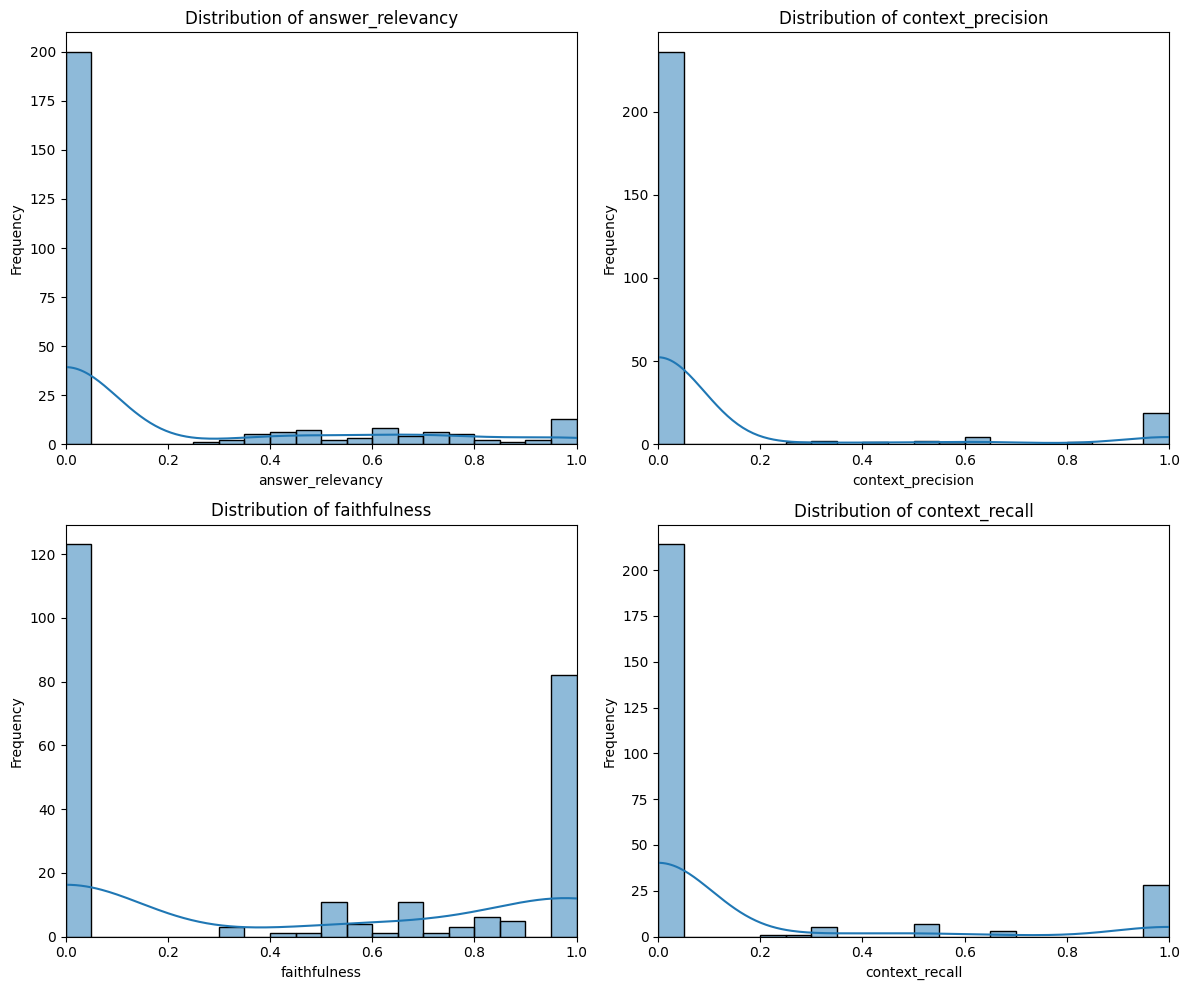
\includegraphics[width=0.7\textwidth]{images/3_3_code_invest_D_D.png}
    \caption{DeepSeek Ergebnis für 300 Fragen (mit Code-Dokumenten)}
    \label{fig:deepseek_code}
\end{figure}

\begin{figure}[htbp]
    \centering
    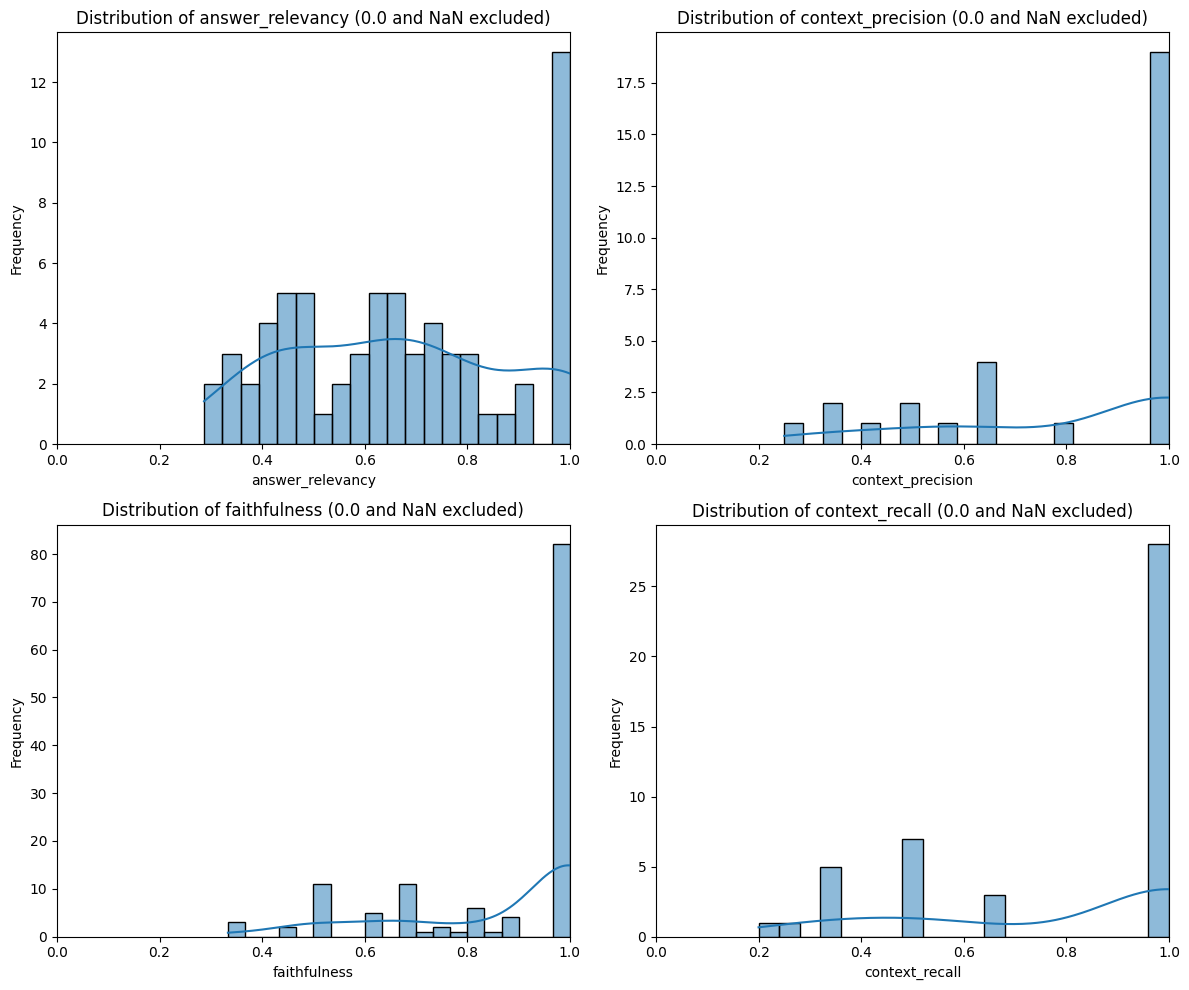
\includegraphics[width=0.7\textwidth]{images/127_44_code_invest_O_O.png}
    \caption{ChatGPT Ergebnis für 300 Fragen (mit Code-Dokumenten)}
    \label{fig:chatgpt_code}
\end{figure}
Der Vergleich der Anzahl der 0.0-Bewertungen mit DeepSeek (Abbildung \ref{fig:deepseek_code}) im Vergleich zu OpenAI (Abbildung \ref{fig:chatgpt_code}) ist eindeutig.

106 (~40\,\%) der insgesamt 276 zu bewertenden Fragen waren mit komplett 0.0 bewertet worden. Bei der Analyse der speziellen Zeichen im Kontext fällt auf, dass 89 Bewertungen (~83\,\%) zu mehr als 5\,\% nur aus diesen bestehen. Dies deutet darauf hin, dass DeepSeek starke Probleme hat, Fragen mit Code zu generieren und/oder zu finden.
\begin{figure}[htbp]
    \centering
    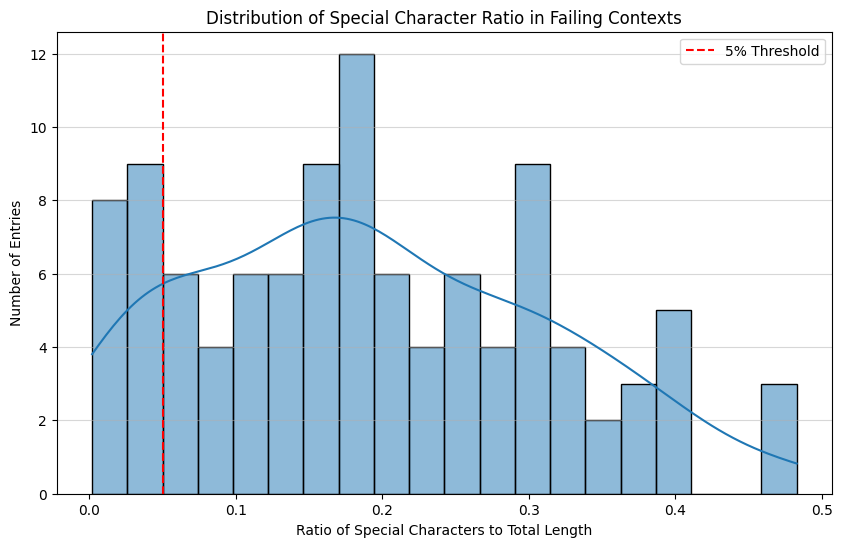
\includegraphics[width=0.8\textwidth]{images/3_3_special_characters.png}
    \caption{Abweichungen des Faithfulness Scores bei Code-Dokumenten.}
    \label{fig:special_characters}
\end{figure}

Ein großer Teil der Fragen hat sich also auf Dokumente mit minderwertiger Qualität, bezogen. Durch diese minderwertigen Dokumente hat sich das LLM dann verwirren lassen.
Es zeigt sich wieder einmal, dass die Qualität der Daten eine entscheidende Rolle spielt!
Bei betrachtung der Ergebnisse ohne Dokumente, welche Code enthalten, sehen wir, dass die 0.0-Bewertungen bei DeepSeek deutlich zurückgehen. Wie zu erwarten war, ist OpenAI's ChatGPT-4 immer noch deutlich besser.

\begin{figure}[htbp]
    \centering
    \begin{minipage}[b]{0.48\textwidth}
        \centering
        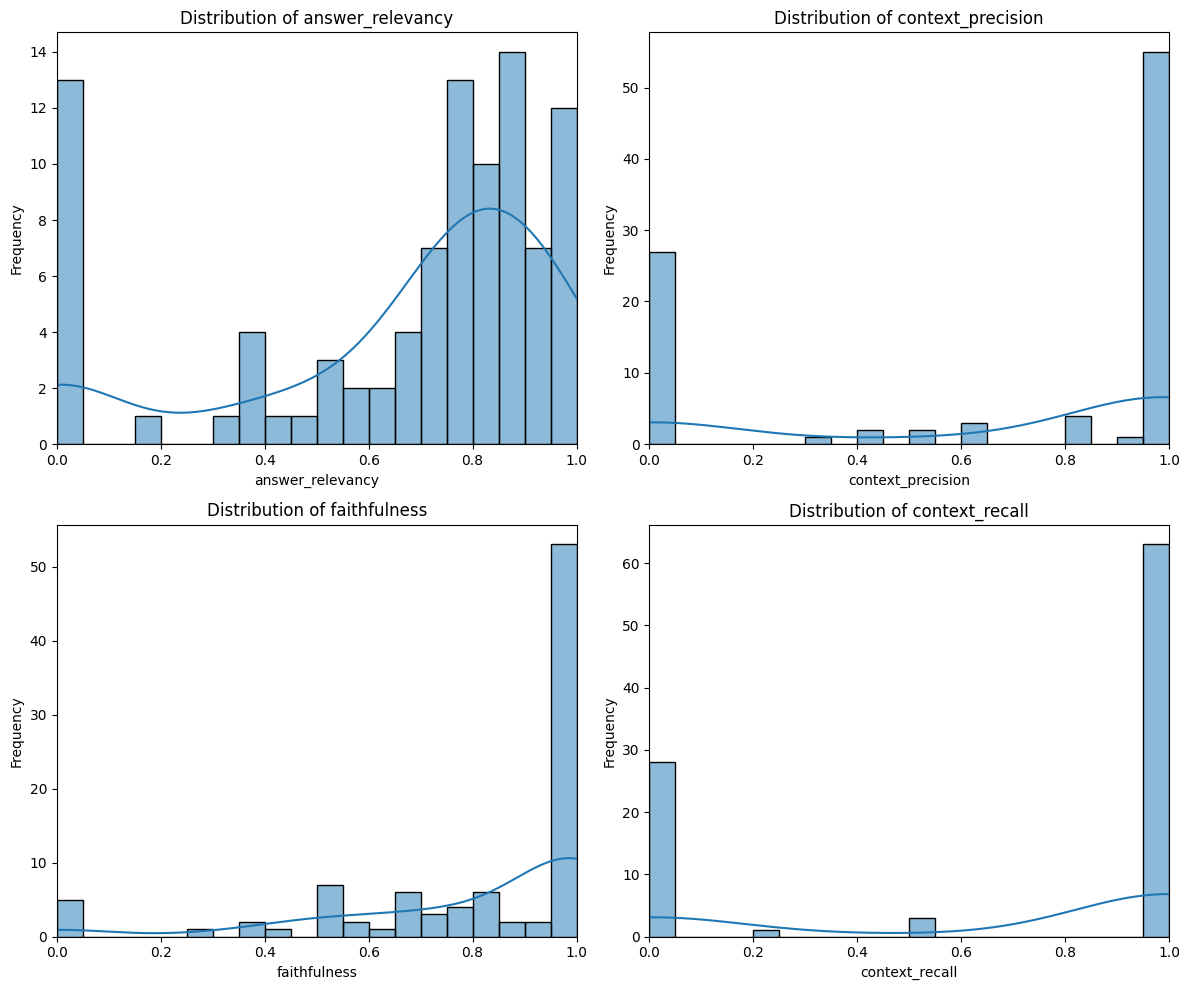
\includegraphics[width=\textwidth]{images/20_4_D_D_distribution.png}
        \caption{DeepSeek Ergebnis für 100 Fragen (ohne Code-Dokumente)}
        \label{fig:deepseek_no_code}
    \end{minipage}
    \hfill
    \begin{minipage}[b]{0.48\textwidth}
        \centering
        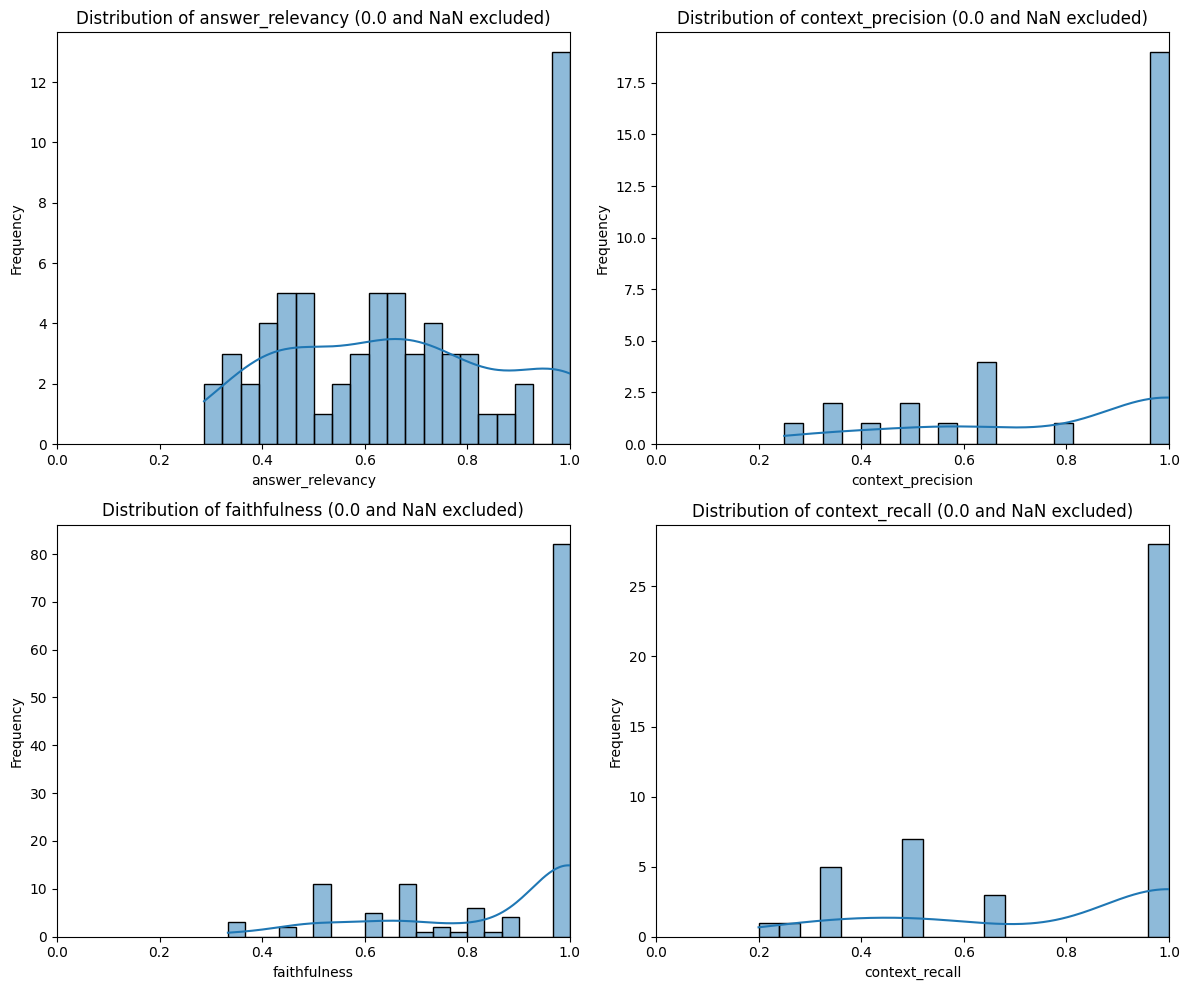
\includegraphics[width=\textwidth]{images/127_38_O_O_distribution.png}
        \caption{ChatGPT Ergebnis für 100 Fragen (ohne Code-Dokumente)}
        \label{fig:chatgpt_no_code}
    \end{minipage}
\end{figure}

---

\subsection{Unterschiede über mehrere Durchläufe}

Um zu prüfen, wie sich die Ergebnisse von Durchlauf zu Durchlauf unterscheiden, wurden für das Testset mit 100 Fragen für 100 Dokumente mit beiden Modellen vier Durchläufe vorgenommen.
In diesem Versuch geht es dann die Unterschiede pro Durchlauf für das Modell festzustellen und nicht die Modelle miteinander zu vergleichen.

\begin{figure}[h!]
    \centering
    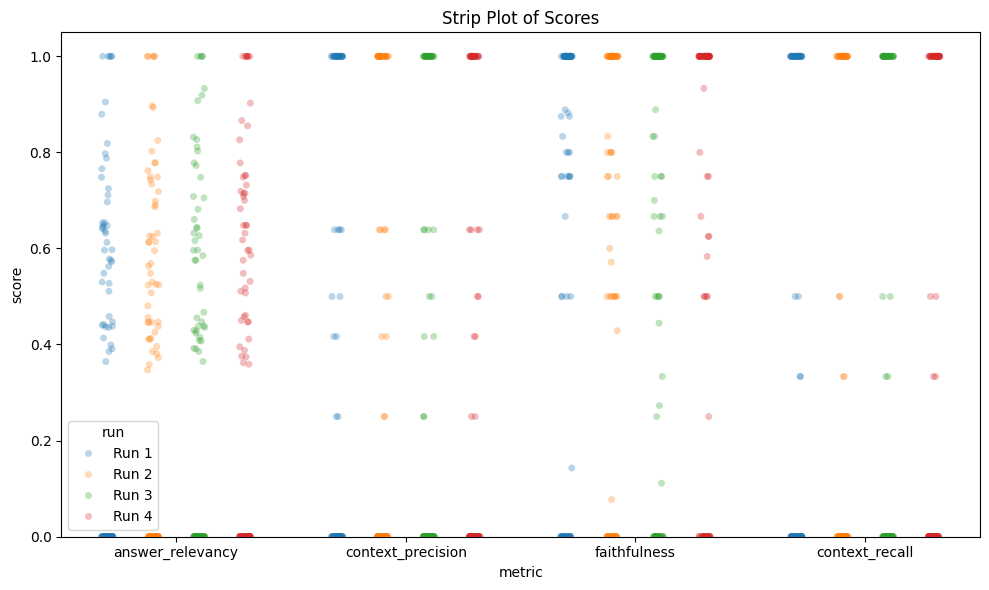
\includegraphics[width=0.9\textwidth]{images/strip_plot_100_100_D_D.png}
    \caption{Bewertung der vier Durchläufe mit DeepSeek}
    \label{fig:strip_plot_deepseek}
\end{figure}

\begin{figure}[h!]
    \centering
    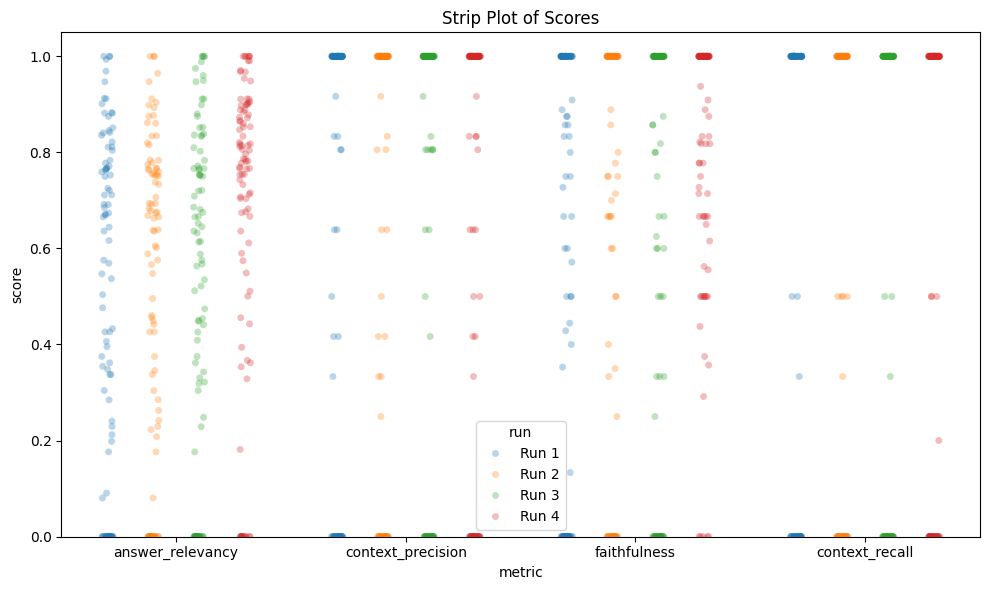
\includegraphics[width=0.9\textwidth]{images/strip_plot_100_100_O_O.png}
    \caption{Bewertung der vier Durchläufe mit GPT-4}
    \label{fig:strip_plot_gpt4}
\end{figure}

Beim Betrachten der Strip Plots lässt sich gut sehen, dass die Verteilung der Werte pro Durchlauf sehr ähnlich ist und keine großen Abweichungen erkennbar sind.
Der Mean und Std wurde über alle Fragen hinweg berechnet.

\begin{table}[h!]
    \centering
    \resizebox{\textwidth}{!}{%
    \begin{tabular}{|l|c|c|c|c|c|c|c|c|}
    \hline
    \textbf{Metrik} & \textbf{Mean 1} & \textbf{Mean 2} & \textbf{Mean 3} & \textbf{Mean 4} & \textbf{Std 1} & \textbf{Std 2} & \textbf{Std 3} & \textbf{Std 4} \\
    \hline
    Answer Relevancy    & 0.336 & 0.366 & 0.329 & 0.358 & 0.346 & 0.340 & 0.347 & 0.361 \\
    Faithfulness         & 0.624 & 0.593 & 0.627 & 0.623 & 0.442 & 0.429 & 0.436 & 0.453 \\
    Context Precision    & 0.344 & 0.344 & 0.344 & 0.344 & 0.449 & 0.449 & 0.449 & 0.449 \\
    Context Recall       & 0.415 & 0.415 & 0.415 & 0.415 & 0.484 & 0.484 & 0.484 & 0.484 \\
    \hline
    \end{tabular}%
    }
    \caption{Durchschnittswerte und Standardabweichungen der Metriken über vier Durchläufe für DeepSeek}
\end{table}

Beim Betrachten des Durchschnitts und der Standardabweichung lässt sich für die Answer Relevancy und die Faithfulness sehen, dass eine gewisse Schwankung vorhanden ist. Die Metriken für den Kontext sind jedoch sehr konstant!\\
Bei der Answer Relevancy lässt sich ein Unterschied von 3.7\,\% feststellen, bei der Faithfulness 3.1\,\%. Dies liegt für vier Durchläufe im Rahmen, bedeutet aber auch, dass dies beim Einrichten einer automatischen Pipeline berücksichtigt werden sollte.

\begin{table}[h!]
    \centering
    \resizebox{\textwidth}{!}{%
    \begin{tabular}{|l|c|c|c|c|c|c|c|c|}
    \hline
    \textbf{Metrik} & \textbf{Mean 1} & \textbf{Mean 2} & \textbf{Mean 3} & \textbf{Mean 4} & \textbf{Std 1} & \textbf{Std 2} & \textbf{Std 3} & \textbf{Std 4} \\
    \hline
    Answer Relevancy    & 0.680 & 0.681 & 0.666 & 0.667 & 0.320 & 0.314 & 0.315 & 0.313 \\
    Context Precision    & 0.671 & 0.670 & 0.666 & 0.667 & 0.443 & 0.445 & 0.444 & 0.445 \\
    Context Recall       & 0.647 & 0.671 & 0.681 & 0.665 & 0.472 & 0.456 & 0.458 & 0.461 \\
    Faithfulness         & 0.846 & 0.800 & 0.815 & 0.823 & 0.247 & 0.295 & 0.273 & 0.295 \\
    \hline
    \end{tabular}%
    }
    \caption{Durchschnittswerte und Standardabweichungen der Metriken über vier Durchläufe für GPT-4}
\end{table}

Beim Betrachten des Durchschnitts und der Standardabweichung zeigt sich, dass GPT-4 insgesamt eine konstante Leistung liefert. Die Werte für Answer Relevancy bewegen sich zwischen 66.6\,\% und 68.1\,\%, was einer Abweichung von lediglich 1.5\,\% entspricht. Auch die Standardabweichung ist mit etwa 0{,}31 gleichmäßig verteilt.

Bei der Faithfulness sind die Mittelwerte etwas variabler und reichen von 80.0\,\% bis 84.6\,\%. Dies ergibt eine Differenz von 4.6\,\%, die im Rahmen liegt, aber auf gewisse inhaltliche Schwankungen hinweist.

Die Metriken für den Kontext (Context Precision und Context Recall) zeigen ebenfalls eine stabile Entwicklung mit geringen Unterschieden in den Mittelwerten. Die Standardabweichungen sind bei diesen Metriken nahezu konstant.

Insgesamt zeigt GPT-4 verlässliche Ergebnisse mit nur geringen Varianzen über mehrere Durchläufe hinweg. 


\subsection{Zuverlässigkeit von Metriken}

Um genauer zu untersuchen, wie sich die Metriken bei mehrfacher Ausführung verhalten, wurden die vier Metriken jeweils 50 Mal ausgeführt.
Bei der Bewertung wurde immer GPT-4.1 verwendet.

\subsubsection{Context Precision \& Recall}
Beide Metriken wurden 50 Mal bewertet und haben sich wie bei DeepSeek in der Gesamtbewertung als sehr stabil herausgestellt. Es gab in keinem der Durchläufe eine Abweichung.

\subsubsection{Answer Relevancy}
Hier wurden minimale Abweichungen festgestellt; diese belaufen sich aber auf die zweite Nachkommastelle in der Prozentangabe und sind daher vernachlässigbar.

\begin{figure}[htbp]
    \centering
    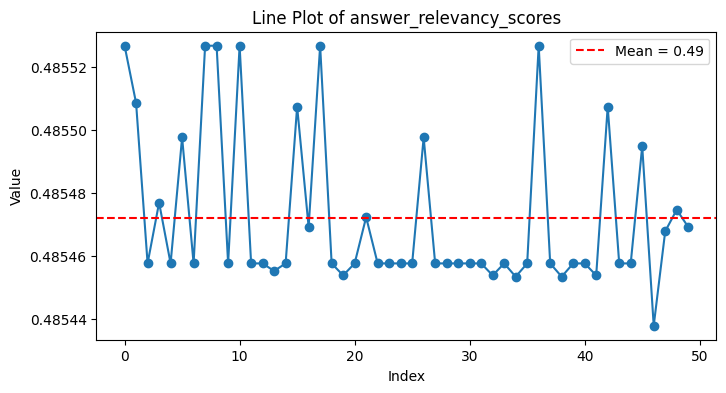
\includegraphics[width=0.8\textwidth]{images/answer_relevancy.png}
    \caption{Abweichungen des Answer Relevancy Scores.}
    \label{fig:answer_relevancy_deviation}
\end{figure}

\subsubsection{Faithfulness}
Bei der Faithfulness sieht dies schon etwas anders aus. Die richtige Bewertung wäre 62.5\,\%. In 66\,\% der Fälle war dem auch so, es ist jedoch ersichtlich, dass der Wert teilweise bis zu 12.5\,\% abweichen kann.

\begin{figure}[htbp]
    \centering
    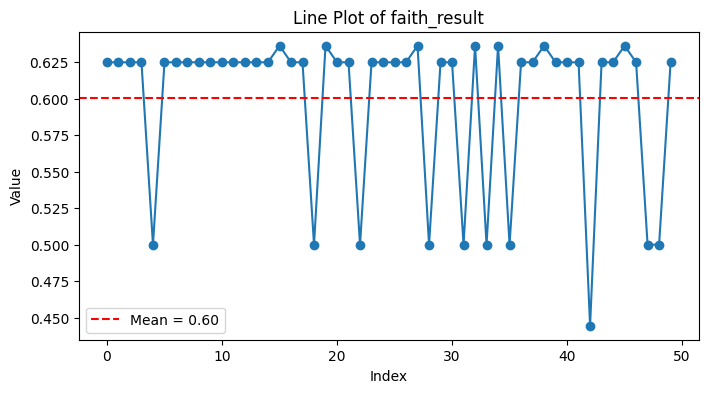
\includegraphics[width=0.8\textwidth]{images/faithfullness.png}
    \caption{Abweichungen des Faithfulness Scores.}
    \label{fig:faithfulness_deviation}
\end{figure}

Die Faithfulness-Metrik hat die größten Schwankungen; dies war auch schon bei dem Versuch mit mehreren Durchläufen ersichtlich.

\subsubsection{Ausführungszeiten DeepSeek}
Da es bei OpenAI zu den Rate Limits kommen kann, wurde die Anzahl an gleichzeitigen Abfragen von 16 auf 1 reduziert, da es sonst besonders bei längeren Durchläufen zu Problemen kommt.
Das führt zu einer deutlichen Verschlechterung der Ausführungszeit.
Das Generieren des Testsets mit 15 Fragen dauerte bei 16 gleichzeitigen Anfragen 2 Minuten, bei nur einer maximalen Anfrage wurden es 7 Minuten.
Mit diesen Zahlen lässt sich annehmen, dass der Versuch mit 300 Fragen ohne Rate Limit seitens OpenAI sicherlich unter einer Stunde geschafft werden könnte.

\begin{table}[h!]
    \centering
    \begin{tabular}{|c|c|}
    \hline
    \textbf{Anzahl} & \textbf{Dauer (hh:mm)} \\
    \hline
    15   & 00:02 \\
    30   & 00:03 \\
    50   & 00:04 \\
    100  & 00:07 \\
    150  & 01:37 \\
    300  & 02:30 \\
    \hline
    \end{tabular}
    \caption{Dauer der Evaluation pro Dokumentenanzahl mit DeepSeek}
\end{table}

\subsubsection{Ausführungszeiten OpenAI}
Für die Bewertung des Testsets mit 300 Fragen (400 Dokumente) wurde Tracing genutzt. Dies lässt uns genauer prüfen, warum gewisse Bewertungen fehlgeschlagen sind.
Es kam insgesamt zu 20 Fehlern: 12 Zeitüberschreitungen, weil das LLM nicht innerhalb von 10 Minuten geantwortet hat, acht Antworten waren in einem ungültigen Format, sieben davon für context\_recall und eine für faithfulness.
Mit den 20 fehlgeschlagenen Metriken kommen wir auf eine \textbf{Fehlerquote} von 1.9\,\%.

\begin{table}[h!]
    \centering
    \begin{tabular}{|c|c|}
    \hline
    \textbf{Anzahl} & \textbf{Dauer (hh:mm)} \\
    \hline
    15   & 00:41 \\
    30   & 01:03 \\
    50   & 01:35 \\
    100  & 03:41 \\
    150  & 05:20 \\
    300  & 17:29 \\
    \hline
    \end{tabular}
    \caption{Dauer der Evaluation pro Dokumentenanzahl mit OpenAI}
\end{table}

\subsection{Kostenberechnung}

Die Bewertung des RAGs mit den 300 Fragen und OpenAI hat 2 Stunden und 30 Minuten gedauert, dabei sind Kosten in Höhe von 12 Euro entstanden.

Dies kann man mit einer Bewertung, wie in den Versuchen, auf einem Mac Studio (M2 Ultra) vergleichen.
\begin{itemize}
    \item Laufzeit pro Bewertung DeepSeek: 17\,h
    \item Stromkosten: 0,12\,\texteuro/h $\Rightarrow$ 17\,h $\times$ 0,12\,\texteuro/h = \textbf{2,04\,\texteuro}
    \item OpenAI API-Kosten pro Bewertung: 12,00\,\texteuro\\
          Davon sollen 2,00\,\texteuro lokal durch eigene Ausführung ersetzt werden $\Rightarrow$ verbleibende Abschreibung: \textbf{10,00\,\texteuro/Run}
    \item Geräteanschaffung: 7.200\,\texteuro $\Rightarrow$ amortisiert über 720 Runs à 10,00\,\texteuro
    \item Gesamtkosten pro Run: 2,04\,\texteuro (Strom) + 10,00\,\texteuro (Abschreibung) = \textbf{12,04\,\texteuro}
    \item Gesamtlaufzeit (720 Runs): 720 $\times$ 17\,h = 12.240\,h $\approx$ \textbf{1 Jahr, 4 Monate, 10 Tage}
\end{itemize}

Die Preise für die Nutzung eines LLMs über eine Schnittstelle zu entscheiden liegt hier komplett beim Anbieter.
Auch die Preise für Strom oder Hochleistungs-GPUs können in Zukunft schwanken.
Sollte es also in Zukunft Änderungen an diesen variablen Preisen geben könnte diese Entscheidung anders ausfallen.

\section{Abhängigkeit der Metriken untereinander}
Die Metriken für den Kontext finden früher im Ablauf einer Anfrage an das RAG statt. Sollten diese Metriken als besonders gut order schlecht sein, lässt sich deutlich sehen, wie sich dies auf die danach folgenden Metriken auswirkt.

\begin{figure}[htbp]
    \centering
    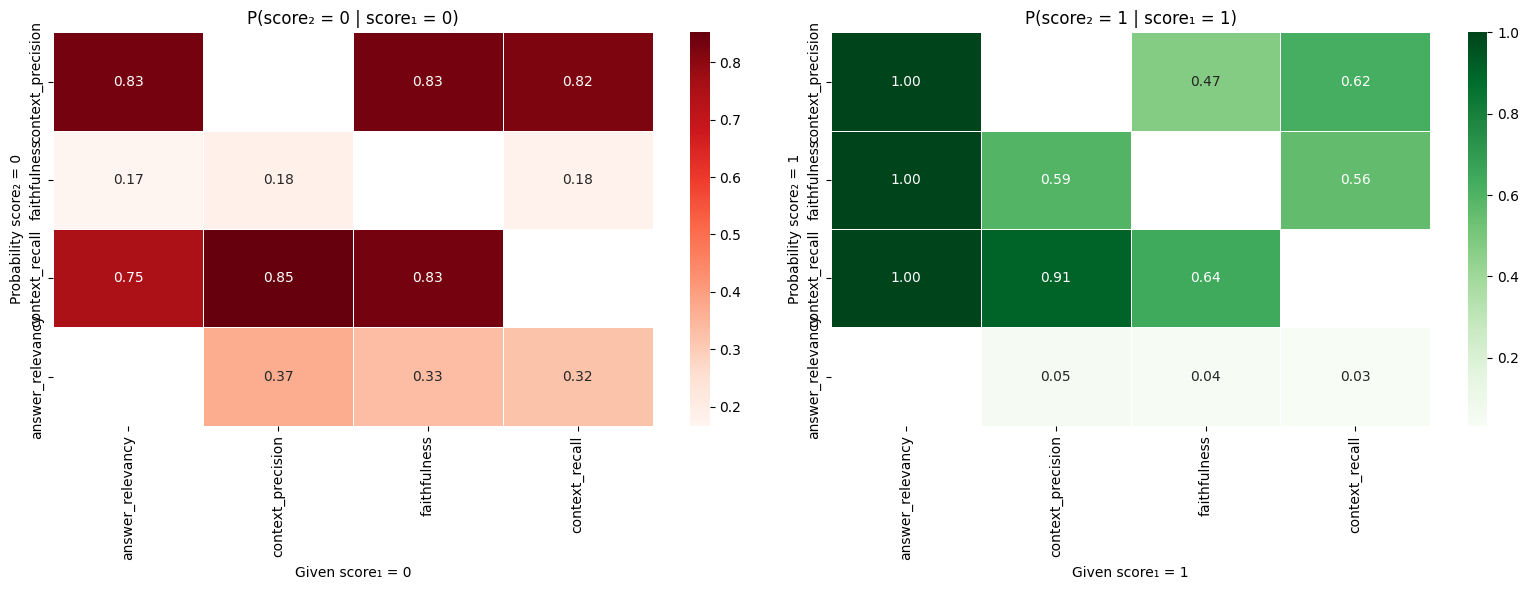
\includegraphics[width=0.8\textwidth]{images/metric_influence_400_300_O_O.png}
    \caption{Abhängigkeit der Metriken voneinander (OpenAI, 300 Fragen, 400 Dokumente)}
    \label{fig:metric_influence}
\end{figure}

Wenn die Metriken für den Kontext (context\_precision und context\_recall) eine Bewertung von 0 haben, ist die Wahrscheinlichkeit, dass die anderen Metriken auch 0 sind, relativ hoch.
In diesem konkreten Beispiel werden die Abhängigkeiten des OpenAI RAGs für die 300 Fragen gezeigt. Es lässt sich sehen, dass die faithfulness deutlich weniger von den Kontext-Metriken abhängt.

In der finalen Auswertung sollten Anwender also überlegen, Metriken wie Answere Accuracy besonders zu betrachten, wenn die Context Metriken gut bewertet worden sind.